\chapter{Minimization of a Functional}
	
	A classical problem in minimization is the brachistrochrone, so the fastest ultimate curve (meaning determining the fastest trajectory to move from a point $A$ to a point $B$ considering that the only action is the one of the gravity).
	
	\textbf{MAGARI FARE LA FIGURA}
	
	Mathematically the problem is determining the curve $\mathcal C: [a,b] \rightarrow \mathds R$ such that $\mathcal C(a) = y_a$ and $\mathcal C(b) = y_b$ that minimize the function $T(\mathcal C)$ representing the time to travel and so
	\[ \textrm{minimize } T(\mathcal C) \qquad \textrm{for all possible curves } \mathcal C \]
	
	We can see that a \textbf{function} takes a number as input and returns a number, like $f(x) = x e^x$. A \de{functional} is instead something that takes as input a function and returns a number and an example is
	\[ \mathcal F (x) = \int_a^b x(t)\, dt  \]
	where $x$ is a function. Considering for example $x(t) = t^2$ the previous functional  becomes
	\[ \fun F(x) = \int_a^b t^2\, dt = \left. \frac{t^3}{3}\right|_a^b= \frac{b^3-a^3}{3}\]
	
	Another example of functional can be $\fun G(z) = z'(0) \int_0^1 z^2(t)\, dt$ and this expression can be evaluated for every generic function $z(t)$.	\vspace{3mm}
	
	The question of this problem is how to define a \textit{minimum} for a functional; in order to do so we have to firstly understand how to minimize a simple function and in particular given a function $f: A\subseteq \R \rightarrow \R$ has a minimum in the point $x^*$ if
	\[  f(x^*) \leq f(x) \qquad \forall x \in A \]
	Similarly given a function $\fun F(x)$ a \textit{point} $x^*$ (that in reality is a function) is a minimum if 
	\[ \fun F(x^*) \leq \fun F(x) \qquad \forall x \in ? \]
	In this case we have to specify the \textit{class} (functional space) of functions we are considering, as example $x$ can be a function that's continuous in the domain $[a,b]$ and so we can define
	\[ x\in C([a,b]) = \big\{ g:[a,b]\rightarrow R \ | \ g \textrm{ is continuous} \big\} \]
	In general changing the \textit{domain} of the functional $\fun F$ may change the problem.
	\begin{example}{: domain change}
		Considering the function $f(x) = x^2+2$, it's roots can be computed if we allow complex solutions $z\in \mathds C$ (and in fact $z = \pm i \sqrt 2$), while if the domain of the solution is the real set $z\in \R$ no solutions exists. \vspace{3mm}
		
		Considering now the functional $\fun F$ defined as
		\[ \fun F(x) = \int_{-1}^1 \big(x(t) - |t|\big)^2\, dt \]
		The $|t|$ introduce a cuspid in $t=0$ that cannot be derived. If we minimize the functional in the continuous interval $x\in C([-1,1])$, the solution is the function $x^*(t) = |t|$, in fact
		\[ \fun F(x^*) = \int_{-1}^1 \big(|t|-|t|\big)^2 \, dt = \int_{-1}^1 0\, dt = 0 \]
		Choosing any other continuous function will result in a functional with a positive value.
		
		Considering now to minimize the function in the domain of functions with continuous derivatives, and so $x\in C^1([-1,1])$. In this case $|t|\notin C^1([-1,1])$ (due to the cuspid). An approximation of the function $|t|$ that is continuous with also continuous first derivative is the function
		\[ x_\varepsilon(t) = \begin{cases}
			t \qquad & t \geq \varepsilon \\
			\frac 1 2 \left(\frac{t^2}\varepsilon + \varepsilon\right) \qquad & -\varepsilon < t< \varepsilon \\
			-t & t \leq- \varepsilon
		\end{cases} \]
		By pushing the limit $\varepsilon\rightarrow 0$ we can have the function that minimize the functional $\fun F$ in the domain $C^1([-1,1])$. In fact we can see that the functional of $x_\varepsilon$ becomes
		\[ \fun F(x_\varepsilon) = \int_{-\varepsilon}^\varepsilon \left( \frac{t^2}{2\varepsilon} + \frac \varepsilon 2 - |t| \right)^2\, dt = \frac{\varepsilon^3}{10} \]
		
	\end{example}

\section{Analogies with linear algebra}
	To solve the problem of minimizing a functional we can see some relations with the linear algebra. The domain of the functional can be in fact see as a \de{functional space} $\mathds V$ analogous to the vectorial one which the vectors are represented by the functions and the scalars are represented by real values. With this definition example of functional spaces might be
	\[ \mathds V_1 = \big\{ f : [0,1] \rightarrow \R \textrm{ continuous}\big\} \]
	\[ \mathds V_2 = \big\{ f: [a,b]\rightarrow \R \textrm{ such that } f\in C^k([a,b]) \big\} \qquad \textrm{with } a,b \in \R, \ k\in \mathds N \]
	Given in fact two function $f,g \in \mathds V$ that are member of the same functional space, we can see that each linear combination of the functions determine a function that's still in the vectorial space:
	\[ \alpha f(x) + \beta f(x) \in \mathds V \qquad \forall \alpha,\beta \in \R, \ f(x),g(x) \in \mathds V \]
	As example let's consider the two continuous function $f(x) = x^2$ and $g(x) = \sin x$, then we can clearly see that the function $2f(x) + \frac 13 g(x) = 2x^2 +\frac 13\sin x$ is still continuous. This in general means that the functional space is \textit{closed} respect to the operations of function summation and multiplication by a scalar.
	
	\paragraph{Scalar product} In linear algebra given two vector $\vett v_1, \vett v_2$ it exists the bilinear operator scalar product $\langle \vett v_1,\vett v_2 \rangle = \vett v_1 \cdot \vett v_2$  that satisfy the following rules:
	\[ \langle \alpha \vett v + \beta \vett w, \vett z\rangle = \langle \vett z , \alpha \vett v + \beta \vett w\rangle = \alpha \langle \vett v,\vett z\rangle + \beta \langle \vett w,\vett z\rangle \qquad \forall \alpha,\beta \in \R, \ \vett v,\vett w,\vett z \in \mathds V \]	
	\[ \langle \vett v,\vett v\rangle \geq 0 \qquad \textrm{ and } \qquad \langle \vett v,\vett v \rangle = 0 \quad \Leftrightarrow \quad \vett v = \vett 0 \]
	
	Also in the functional space $\mathds V$ can exists definitions of product scalar such the one here presented:
	\begin{equation} \label{eq:func:pscalexample}
		\langle f,g\rangle = \int_0^1 f(x)g(x)\, dx
	\end{equation}
	\begin{note}
		This is not the lonely function that can serve as product scalar of function and in this case the relation holds for the functional space $\mathds V = \{ f:[0,1] \rightarrow \R \textrm{ integrable} \}$.
	\end{note}
	In this case we can prove that this definitions meets the requirements stated for the scalar product considering the linear properties of the integrals as follows:
	\begin{align*}
		\langle \alpha f(x) + \beta g(x),h(x) \rangle & = \int_0^1 \Big(\alpha f(x) + \beta g(x)\Big)h(x) \, dx \\ 
		& = \alpha \int_0^1 f(x)h(g) \, dx + \beta \int_0^2 g(x)h(x) \, dx \\
		& = \alpha \langle f(x),h(x) \rangle + \beta \langle g(x),h(x) \rangle
	\end{align*}
	and also
	\[ \langle f(x),f(x) \rangle = \int_0^1 f(x) f(x) \, dx = \int_0^1 f^2(x)  \geq 0  \]
	and in particular we can see that the scalar product $\langle f(x),f(x)\rangle$ will give as result 0 if and only if the function $f$ is identically null, so such that $f(x) = 0$ for all $x$ in it's domain (in this case $[0,1]$).
	
	\paragraph{Norm} In linear algebra it's also defined the norm of a vector as
	\[ \|\vett v\| := \sqrt{\vett v \cdot \vett v} \]
	and this expression is used to compute, from a vector, a single positive value  (and in particular $\|\vett v\| = 0$ if and only if $\vett v = \vett 0$). This definition also holds for the functional space and considering the scalar product defined (as example) in equation \ref{eq:func:pscalexample} we can see that one definition of norm for function can be the one
	\[ \|f(x)\| = \sqrt{\langle f(x),f(x)\rangle} = \sqrt{\int_0^1f^2(x) \, dx} \]
	In this case we can clearly see that the norm $\|f(x)\| \geq 0$ is always positive defined (and is zero only in the case on which the function $f$ is identically null).
	
	
	\begin{example}{: space of function}
		A space of functions can ve the one $f:[a,b]\rightarrow \R$ such that $f$ is continuous, or for example $f:[a,b]\rightarrow \R$ where $f\in C^k([a,b])$ (for $k\in \mathds N$). The same can be said for piecewise continuous functions.
		
		Less trivially is a space of function the set of $f:[a,b]\rightarrow \R$ that are module integrable, and so all the function $f$ such that
		\[\int_a^b |f(x)|\, dx < \infty\]
		
	\end{example}

	In general we define as $L^p([a,b])$ the space of $p$-integrable functions, so such that
	\[ f\in L^p([a,b])  \qquad \Leftrightarrow \qquad \int_a^b |f(x)|^p\, dx < \infty\]
	
	
\section{Directional derivative} 
	Given a bidimensional function $f:\R^2\rightarrow \R$ in the variable $x,y$ a point $(x\s,y\s)$ is a global minimum if it satisfy the following relation:
	\[ f(x\s,y\s) \leq f(x,y) \qquad \qquad \forall (x,y)\in \R^2 \]
	
	Given so a direction defined by the vector $\vett d = (dx,dy)$ it's possible to reconduct the multi valued function $f$ into a one dimensional function $g$ as
	\[ g(t) = f\big( x\s + t\, dx,y\s + t\, dy \big)  \]
	With this definition we can see that $g(0)$ corresponds to $f(x\s,y\s)$ and so for any other value of $t$ it happens that $g(t) \geq f(x\s,y\s)$ (based on the assumption that $(x\s,y\s)$ is the global minimum of the function $f$). This also means that the relation $g(t)-g(0) \geq 0$ for all value of $t \geq 0$: dividing this relation by the parameter $t$ and pushing the limit for the variable approaching zero will give the analytical result of the derivative of $g$ evaluated at zero
	\begin{equation} \label{eq:func:directional}
		g'(0) := \lim_{t\rightarrow 0} \frac{g(t) - g(0)}{t} \geq 0 
	\end{equation}
	
	If the function $f$ also presents a Taylor series expansion of the first order respect to the point $(x\s,y\s)$ of global minimum it can be written as
	\[ f\big( x\s + t\, dx, y\s +t \, dy\big) = f\big(x\s,y\s\big) +\nabla f\big(x\s,y\s\big) \vector{t \,dx \\ t\, dy} + \mathcal O(t^2) \]
	Rearranging this expression on the by shifting to the left the term $f(x\s,y\s)$ and dividing by $t$ it's possible to observe the relation to the directional derivative (equation \ref{eq:func:directional}) as
	\begin{align*}
		\frac{g(t)-g(0)}{t} & = \frac{f( x\s + t\, dx, y\s +t \, dy)  - f(x\s,y\s)}{t} \\
		& = \nabla f\big(x\s,y\s) \vector{dx \\ dy} + \cancel{\mathcal O(t)}
	\end{align*}
	As shown previously it must be that the directional derivative $g'(0) = \nabla f(x\s,y\s) \vett d \geq 0$ must be greater or equal to zero. Considering however as direction on which compute the derivative the opposite of the one determined by the gradient, so $\vett d = - \nabla f(x\s ,y\s)^t$, we can see that the product becomes
	\[ \nabla f(x\s,y\s) \big(-\nabla f(x\s,y\s)^t\big) = - \| f(x\s,y\s)\|^2 \]
	We can now see that the lonely way to have $-\|f(x\s,y\s)\geq 0$ is having a function $f$ such that it's gradient  is identically null, and so $\nabla f(x\s,y\s) = \vett 0$.
	
\subsection{Stationary points for a functional}
	Until now we defined a functional $\mathcal F: \mathds V \rightarrow \R$ a type of function that relate function of the functional space $\mathds V$ with real values in $\R$. Let $x\s(t)$ a function that \textit{minimize} the functional $\mathcal F(x)$ and consider $y(t)$ another \textit{point} (function) in the functional domain: this means that
	\[ \F(x\s) \leq \F(y) \]
	
	In this functional space we can determine a line that connects the points determined by $x\s$ and $y$ creating a \textit{linear interpolation}, generating a new function $z(t,\tau)$ as a linear combination of the original points:
	\[ z(t,\tau) :=  x\s(t) + \tau \underbrace{\big( y(t) - x\s(t) \big)}_{=d(t) \textrm{: direction}} \]
	We can see that for $\tau = 0$ the function $z$ reduces to the minimum point $x\s$, while for $\tau = 1$ it matches the other point $y$; the difference $y(t)-x\s(t) = d(t)$ indeed represents the direction on which the two functions combines.
	
	With that said it's possible to compute a \textit{slice} $g(\tau)$ of the original functional $\F$ along the direction determined by the function $z(\cdot,\tau)$ and so
	\begin{equation}
		g(\tau) := \F\big( z(\cdot,\tau) \big) = \F\big(x\s + \tau d\big)
	\end{equation}
	We can see that the function $g$ maps a real value $\tau\in\R$ into another real value, and in particular considering the initial assumption of $x\s$ being a minimal point of $\F$ it means that
	\[ g(0) = \F(x\s) \leq g(\tau) = \F(x\s + \tau d) \]
	Considering this relations and assuming that's possible to compute the derivative of $g$, evaluating it for the point $\tau = 0$ will get the results:
	\begin{align*}
		g'(0) & = \lim_{\tau\rightarrow 0^+} \frac{g(\tau)-g(0)}{\tau} \geq 0 \\
		& = \lim_{\tau\rightarrow 0^-} \frac{g(\tau)-g(0)}{\tau} \leq 0 
	\end{align*}
	and so this means, in order to have a continuous derivative for $\tau = 0$ that the \textbf{derivative must be null}:
	\[ \Rightarrow \qquad g'(0) = 0 \]
	
	The conclusion of this process is that a function $x\s$ to be a minimum point must present a directional derivative that's equal to zero for each feasible direction $d$ that we consider.
	
	
	\begin{example}{: directional derivative of a functional}
		Given the functional
		\[ \fun F(x) = \int_0^1 \Big(x^2(t) + 1\Big) \, dt  \ + x(1) \]
		it's  possible to compute the directional derivative in $x(t)$ with direction $d(t)$ by firstly determining the function $g:\R\rightarrow \R$ that's the evaluation of the functional for the function $z(t,\alpha) = x(t) + \alpha \, d(t)$:
		\begin{align*}
			g(\alpha) & = \F \big(z(t,\alpha)\big) = \F\big(x(t) + \alpha\, d(t)\big) \\
			& = \int_0^1 \Big( \big(x(t) + \alpha\, d(t)\big)^2 + 1 \Big)\, dt  + x(1) + \alpha\, d(1)
		\end{align*}
		Deriving this expression respect to the parameter $\alpha$ will give the function
		\[ g'(\alpha ) = \frac{dg(\alpha)}{d\alpha} = \frac d{d\alpha } \int_0^1 \Big( \big(x(t) + \alpha\, d(t)\big)^2 + 1 \Big)\, dt  +  \frac d{d\alpha} \Big(x(1) + \alpha\, d(1)\Big) \]
		
		Assuming that $\frac d{d\alpha}\int = \int \frac d{d\alpha}$ (operation that cannot always be performed) this expression reduces to a form that's easier to evaluate:
		\begin{align*}
			g'(\alpha) &= \int_0^1 \frac d{d\alpha} \Big(x(t) + \alpha\, d(t)\Big)^2\, dt + \frac d{d\alpha} \Big(x(1) + \alpha \, d(1)\Big) \\
			& = \int_0^1 2\big(x(t) + \alpha\, d(t)\big) d(t)\, dt + d(1) \\
			g'(0)& = \int_0^1 2x(t)d(t)\, dt + d(1)
		\end{align*}
		and so the directional derivative of the original functional $\F$ respect to the direction $d(t)$ is determined by $g(0)$.
	\end{example}
	
\section{Fundamental lemma of the calculus of variations}
	{\itshape Given a function $f:[a,b]\rightarrow \R$ (piecewise continuous) such that for all $g:[a,b] \rightarrow \R$ continuous (and more in particular $g \in C^\infty([a,b])$ to have a more general definition ) with $g(a) = g(b) = 0$ and $g^{(k)}(a) = g^{(k)}(b) = 0 \ \forall k$, if the integral 
	\begin{equation} \label{eq:func:lemma}
		\int_a^b f(x)\,g(x) \, dx = 0
	\end{equation}
	then $f(x)= 0 $ is identically null. }

	\paragraph{Lemma: sign permanence} In order to later proof the fundamental lemma yet described, we have to remark the \textit{sign permanence} that states: {\itshape given a function $f:[a,b]\rightarrow \R$ continuous such that $f(c) >0$, then there exists a $\delta >0$ such that }
	\[ f(x) \geq \frac{f(c)}{2} \qquad \forall x \in [c-\delta,c+\delta] \]
	
	The proof of this lemma can be done defining the parameter $\epsilon = f(c) / 2$; based on the assumption that $f(x)$ is continuous, then
	\[ \exists \delta >0 \qquad \textrm{such that} \qquad |f(x) - f(c)| \leq \varepsilon = \frac{f(c)}{2} \qquad \forall |c-x|\leq \delta \]
	Expanding the module operation the inequality becomes:
	\[ -\frac{f(c)}{2} = - \epsilon \leq f(x)-f(c) \leq \epsilon = \frac{f(c)}{2} \]
	\[ \Rightarrow \qquad \underbrace{-\frac{f(c)}{2} + f(c) \leq f(x)}_{\frac{f(c)}{2} \leq f(x)} \leq f(c) + \frac{f(c)}{2} \]
	and so we prove the lemma of sign permanence.
	
	\paragraph{Proof of the fundamental lemma} The proof of the fundamental lemma of the calculus of variation can be done by contradiction. Let consider the integral $\int_a^b f(x) g(x)\, dx = 0$ for all functions $g(x)$ and such that, given the function $f$, exists a point $c$ such that $f(c) > 0$ (in general the proof can be done for $f(c)\neq 0$). from the sign permanence lemma we can state that exists an interval $[c-\delta,c+\delta]$ such that $f(x) \geq \frac{f(c)}{2 } \geq 0$. Determining the function $g$ as
	\[ g(x) = \begin{cases}
		\dfrac{x-(c-\delta)}{\delta} \qquad & x\in [c-\delta, c] \\
		\dfrac{c-x+\delta}{\delta} & x\in[c,c+\delta] \\
		0 & \textrm{otherwise}
	\end{cases} \]
	Note that this function is continuous but $g\notin C^\infty$ (later will be described a function that presents this feature). With this definition the integral $\int_a^b fg\, dx$ so becomes
	\begin{align*}
		\int_{c-\delta}^{c+\delta} f(x)g(x)\, dx & \geq \frac{f(c)}{2} \int_{c-\delta}^{c+\delta} g(x)\, dx \\
		& \geq \frac{f(c)}{2}\frac \delta 2 > 0
	\end{align*}
	We can clearly see that the integral $\int_a^b fg\, dx$ has a positive real value grater than zero that's (considering that $f$ has at least on point $c$ such that $f(c) >0$) in contraposition with the initial request that the integral should have been zero evaluated. \vspace{3mm}
	
	To create a direction function $g$ that's in the set $C^\infty$ we can use the function $h$(for whose those condition is demonstrated) as in figure \ref{fig:func:ht} defined as:
	\begin{equation} \label{eq:func:ht}
		h(t) = \begin{cases}
			e^{-1/t} \qquad & t > 0 \\ 
			0 & t\leq 0
		\end{cases}
	\end{equation}
	\begin{SCfigure}[2][bt]
		\centering 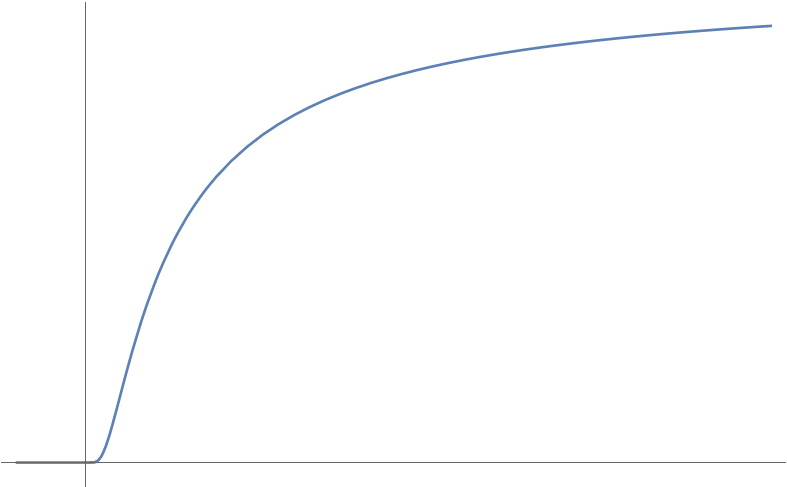
\includegraphics[width=4cm]{cinf-a}
		\caption{representation of $h(t)$ defined in equation \ref{eq:func:ht}}.
		\label{fig:func:ht}
	\end{SCfigure}

	A way to create a function that presents a \textit{bell shape} in the range $[0,1]$ is by computing $g(t) := h(t) h(1-t)$ how's graph in the range $[0,1]$ is similar to the one shown in figure \ref{fig:func:hbell}.
	
	\begin{SCfigure}[2][bht]
		\centering 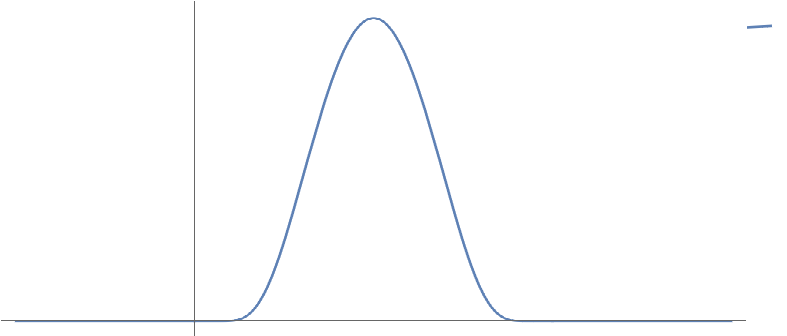
\includegraphics[width=4cm]{cinf-b}
		\caption{representation of the function $g(t):=h(t)h(1-t)$, where $h(t)$ is defined in equation \ref{eq:func:ht}}.
		\label{fig:func:hbell}
	\end{SCfigure}
	
	In particular to demonstrate the fundamental lemma of the calculus of variations we need to rescale the function $g$ in order to have a bell centered in the point $c$ with a \textit{bell width} $\delta$ and so we consider
	\[ g(t) = K \, h\left(\frac{t-c+\delta}{2 \delta}\right) h\left( \frac{\delta + c - t}{2 \delta} \right) \] 
	where the constant $K\in\R$ is such that $g(c)=1$ and $\int_a^bg(x)\, dx$. In this case we can see that $g\in C^\infty$, $g(x) \geq 0 $ for all value $x$ and specifically $g(x) = 0 \, \forall x\notin[c-\delta,c+\delta]$.\\
	The lemma can now be proven by contradiction; as in the previous case if we consider a function $f$ that's not identically null (and in this case we assume that there is at least one point $c$ on which $f$ is positive), then we can state that (for the sign permanence theorem)
	\[ f(x) \geq \frac{f(c)}{2} \qquad \forall x \in [c-\delta,c+\delta] \] 
	We can now see that the original integral $\int_a^b fg\, dx$ is not equal to zero, in fact
	\[ \int_a^b f(x)g(x)\, dx \geq \frac{f(c)}{2}\int_a^bg(x)\, dx > 0 \]
	because $g(x)$ is always greater or equal to zero, determining a non zero value as result as in the previous case.
	
\section{Euler Lagrange equation}
	\paragraph{Pendulum example} The \de{Euler Lagrange equation} is the generalization of the minimum action principle that's used in physics. Considering as a practical example the motion of a pendulum of a mass $m$ that's free to oscillate in respect to a pivot point using a rope of length $l$, the kinetic energy $T$ and the potential term $V$ of the system can be expressed as
	\[ T = \frac 1 2 m v^2 \qquad \qquad \qquad V = mgy \]
	Considering $\theta$ as the angle that the rope determines with the vertical axis, then the we can rewrite the energies as functions of the angular position $\theta$ and velocity $\dot \theta$ as
	\[ T(\theta,\dot \theta) = \frac 1 2 m l^2 \dot\theta^2 \qquad \qquad \qquad V(\theta) = - m gl\sin\theta \]
	
	To solve the dynamic equation $\theta(t)$ of the mechanism we can compute the lagrangian $\mathcal L$ of the system defined as
	\[ \mathcal L(\theta,\dot\theta) = T(\theta,\dot\theta)-V(\theta) = \frac m 2 l^2\dot\theta^2 + lmg\cos\theta \]
	As law that's analyzed in mechanics physics we can state that the solution of the dynamics of the system is the one the function that minimize the \textbf{action} $\mathcal A$ of the system defined as
	\begin{equation} \label{eq:func:action}
		A(\theta) = \int_{t_0}^{t_1} \mathcal L(\theta,\dot\theta)\, dt
	\end{equation}
	where the values $\theta(t_0)= \theta_0$ and $\theta(t_1)=\theta_1$ are known parameters.
	
	In practice to determine the required solution we can use analytical tool to find the trajectory that can then be demonstrated to be the minimum of the action $\mathcal A$ (that's indeed a functional).
	
	However we can also try to analytically determine the function $\theta^*(t)$ that minimize the functional $\fun A(\cdot)$ by computing the directional derivatives. \vspace{3mm}
	
	Let now consider the function $\theta\s(t)$ and a direction $\delta_\theta$ that satisfy $\delta_\theta(t_0)=\delta_\theta(t_1) = 0$, we can then use the fundamental lemma of the calculus of variation to determine the minimal function (considering that the expression \ref{eq:func:action} of the action is comparable to equation \ref{eq:func:lemma} of the lemma).\\
	To determine the minimum point we have in fact to determine the function whose derivative is zero for each direction of approach to the point, and so in this example we need to compute
	\begin{align*}
		\frac{d}{d\alpha} \mathcal A\big(\theta\s + \alpha\, \delta_\theta\big) & = \frac{d}{d\alpha}\int_{t_0}^{t_1} \mathcal L \big( \theta \s + \alpha\, \delta_\theta, \dot\theta\s + \alpha\, \dot \delta_\theta \big) \\
		& = \int_{t_0}^{t_1} \left[\pd{}{\theta} \mathcal L( \dots ) \frac{d}{d\alpha}\big(\theta\s + \alpha \,\delta_\theta\big) +\pd{}{\dot\theta} \mathcal L (\dots) \frac{d}{d\alpha}\big(\dot \theta\s + \alpha \,\dot \delta_\theta\big) \right]\, dt \\
		& = \int_{t_1}^{t_2} \left[ \big(-lmg\sin(\theta\s + \alpha\, \delta_\theta)\big)\delta_\theta + ml^2\big(
		\dot\theta\s + \alpha \, \dot\delta_\theta \big)\, \dot\delta_\theta \right] \, dt
	\end{align*}
	Note that from in the first step we made the implicit assumption that $ \frac d{d\cdot} \int = \int\frac{d}{d\cdot}$ while however this is not always possible. Evaluating the previous expression for $\alpha = 0$ we can state that
	\[ 	\frac{d}{d\alpha} \mathcal A\big(\theta\s + \alpha\, \delta_\theta\big) \Big|_{\alpha = 0} = \int_{t_0}^{t_1} \big(-lmg \sin\theta\s\delta_\theta + ml^2\dot\theta\s \dot\delta_\theta \big) \, dt = 0 \qquad \forall \delta_\theta \]
	Performing an integration by part allows to remove the term $\dot\delta_\theta$ that's hard to determine, and in fact
	\[ \frac{d}{dt}\big( ml^2\dot\theta\s \, \delta_\theta\big) = \frac{d}{dt}\big(ml^2\dot\theta\s\big)\,\delta_\theta + ml^2\dot\theta\s \dot\delta_\theta\]
	\begin{align*}
		\Rightarrow \quad \left. \frac{d\mathcal A}{d\alpha}\right|_{\alpha = 0} & = \int_{t_0}^{t_1}  \left[ - lmg\sin\theta\s - \frac d{dt}\big(ml^2\theta\s\big)^2 \right]\delta_\theta\, dt + \cancel{\big[ ml^2 \dot\theta\s \delta_\theta \big]\Big|_{t_0}^{t_1} } \\
		& = \int_{t_0}^{t_1} \underbrace{\left[ -lmg \sin\theta\s - \frac d{dt}\big(ml^2 \dot\theta\s\big) \right]}_{f(t)} \delta_\theta\, dt = 0
	\end{align*}
	We can now see in this formulation that the marked expression represent the function $f$ of the fundamental lemma considering that the relation must be true for all approaching direction $\delta_\theta$, and so it must be
	\[ -lmg \sin\theta\s - \frac d{dt}\big(ml^2 \dot\theta\s\big) = 0 \]
	The problem now to complete the analyses of the pendulum motion is determining the function $\theta\s(t)$ that satisfy this expression and also match the boundary conditions $\theta(t_0) = \theta_0$ and $\theta(t_1)=\theta_1$.
	
\subsection{General formulation}
	Given a functional
	\begin{equation}
		\mathcal A(x) = \int_a^b \mathcal L\big(x(t),x'(t),t\big)\, dt
	\end{equation}
	the problem is to minimize the functional $\mathcal A$ for a function $x \in \mathds V$ such that $x(a) = x_a$ and $x(b) = x_b$ where the function space $\mathds V$ is defined as
	\[ \mathds V = \big\{ x \ | \ x\in C^2([a,b]) \textrm{ with } x(a) = x_a,x(b) = x_b \big\} \]
	Let $\mathds D$ the function space of all the feasible directions of derivatives defined as
	\[ \mathds D = \big\{ \delta_x \ | \ \delta_x \in C^{\infty}([a,b]) \textrm{ with } \delta_x(a) = \delta_x(b) = 0 \big\} \]
	the function $x(t)$ that minimize the functional is the one whose derivative respect to $\alpha$ is always zero (for $\alpha = 0$) for any feasible direction for the derivative, and so 
	\[ x(t) \quad\textrm{such that} \quad \frac{d}{d\alpha} \mathcal{A}(x+\alpha\, \delta_x) \Big|_{\alpha = 0} = 0 \qquad \forall \delta_x \in \mathds D \]	
	
	Assuming the possibility to correctly apply the rule $\frac{d}{d\cdot} \int = \int \frac{d}{d\cdot}$ we can express the derivative of the functional $\mathcal A$ evaluated in $x+ \alpha\, \delta_x$ as
	\begin{align*}
		\frac{d\mathcal A}{d\alpha} & = \frac{d}{d\alpha} \int_a^b \mathcal L\big( x + \alpha\, \delta_x ,x' + \alpha\, \delta_x', t\big)\, dt \\
		& = \int_a^b \left(\pd{\mathcal L}x \delta_x + \pd{\mathcal L}{x'} \delta_x'\right)\, dt \\
		\left. \frac{d\mathcal A}{d\alpha} \right|_{\alpha = 0} & = \int_a^b \left( \pd{\mathcal L(x,x',t)}x \delta_x + \pd{\mathcal L(x,x',t)}{x'} \delta_x' \right)\, dt 
	\end{align*}
	By performing the integration by part it's possible do reconvert the term associated do $\delta_x'$ into pieces depending on $\delta_x$ one of which, when evaluated, becomes zero due to the fact that $\delta_x(a) = \delta_x(b) = 0$:
	\begin{align*}
		\left. \frac{d\mathcal A}{d\alpha} \right|_{\alpha = 0} & = \int_a^b \left[ \pd{\mathcal L(x,x',t)}{x} - \frac{d}{dt} \left( \pd{\mathcal L(x,x',t)}{x'} \right) \right] \delta_x\, dt + \int_a^b\frac{d}{dt}\left( \pd{\mathcal L(x,x',t)}{x'}\delta_x \right) \, dt \\
		& = \int_a^b \left[ \pd{\mathcal L(x,x',t)}{x} - \frac{d}{dt} \left( \pd{\mathcal L(x,x',t)}{x'} \right) \right] \delta_x\, dt + \cancel{\left. \left[ \pd{\mathcal L(x,x',t)}{x'}\delta_x \right] \right|_{\delta_x = a}^b} \\
	\end{align*}
	We can now see that the condition to have a minimum for the functional $\mathcal A$, by using the fundamental lemma of calculus of variation, is requiring that the function $f$ defined as follows is identically null:
	\begin{equation}
		\left. \frac{d\mathcal A(x+\alpha\, \delta_x)}{d\alpha} \right|_{\alpha = 0} = \int_a^b \underbrace{\left(\pd{\mathcal L}{x} - \frac d{dt}\pd{\mathcal L}{x'}\right)}_{=f} \delta_x \, dt = 0
	\end{equation}
	
	This in general means that the function that minimise the functional $\mathcal A$ must solve the following second order ordinary differential equation:
	\[ \begin{cases}
		\dfrac d{dt} \dfrac{\partial\mathcal L}{\partial x'} - \dfrac {\partial \mathcal L}{\partial x} = 0 \\ x(a) = x_a \, ,\ x(b) = x_b
	\end{cases} \]
	
	\paragraph{Definitions} Given a functional $\F$ we define the directional derivative
	\[ \frac{d}{d\alpha} \F(x+\alpha\, \delta_x) \]
	of the functional evaluated on the function $x$ with direction $\delta_x$ as \de{Gateaux derivative} and we simplify the operation of evaluating the derivative for $\alpha= 0$ with the letter $\delta$ as
	\begin{equation}
		\delta \F(x) := \frac{d}{d\alpha} \F\big(x+\alpha\, \delta_x\big) \Big|_{\alpha = 0}
	\end{equation}
	This definition is also referred as the \de{first variation} of the functional $\F(x)$. \vspace{3mm}
	
	Considering now the functional
	\[ \F(x) = \int_a^b \fun G(x,x',t)\, dt + x(a)x(b) \]
	using the \textit{standard} approach until now used, to search for the minimum solution we have to compute the directional derivative evaluating it at the point $\alpha = 0$:
	\begin{align*}
		&= \frac d{d\alpha} \F \big(x+\alpha\, \delta_x\big) \Big|_{\alpha=0} \\
		&= \frac{d}{d\alpha}\left( \int_a^b \mathcal G\big(x+\alpha\, \delta_x, x' + \alpha\, \delta_x',t\big)\, dt  + \Big(x(a) + \alpha \delta_x(a)\Big)\Big(x(b) + \alpha\, \delta_x(b)\Big) \right) \\
		&=  \int_a^b \left( \pd{\mathcal G(\dots)} x \, \delta_x + \pd{\mathcal G(\dots)} {x'} \delta_x' \right) \, dt  + \delta_x(a) \Big(x(b) + \alpha\, \delta_x(b)\Big) + \Big( x(a) + \alpha\,\delta_x(a) \Big)\delta_x(b) \\
		&=  \int_a^b \left( \pd{\mathcal G(\dots)} x \, \delta_x + \pd{\mathcal G(\dots)} {x'} \delta_x' \right) \, dt  + \delta_x(a)x(b) + x(a)\delta_x(b)
	\end{align*}
	Using instead the Gateaux notation for the derivative the same problem can be simplified in the notation as
	\begin{align*}
		&= \delta \F(x) \\
		&= \delta \left(\int_a^b \fun G(x,x',t)\, dt + x(a)x(b)\right) \\
		&= \int_a^b \delta \mathcal G(x,x',t)\, dt + \delta_x(a) x(b) + x(a)\delta_x(b) \\
		&= \int_a^b \left( \pd{\mathcal G(x,x',t)}{x}\delta_x + \pd{\mathcal G(x,x',t)}{x'} \delta_x' \right)\, dt + \delta_x(a) x(b) + x(a)\delta_x(b)
	\end{align*}

\subsection*{Extended definition}
	Considering now the functional $\mathcal B$ defined as
	\[ \mathcal B(x) = \int_a^b \mathcal L(x(t),x'(t),x''(t),t)\, dt \]
	the problem to solve now is the minimization of $\mathcal B(x)$ for all the function $x\in \mathds V$ where the functional space is defined as
	\[ \mathds V = \left\{ x \textrm{ such that } \begin{aligned}
		& x\in C^4([a,b]) \\ & x(a) = x_a, x'(a) = x_a', x(b) = x_b, x'(b) = x_b'
	\end{aligned} \right\} \]
	and directional derivatives $\delta_x \in \mathds D$ in the functional domain
	\[ \mathds D = \left\{ \delta_x \textrm{ such that } \begin{aligned}
		& x\in C^\infty([a,b]) \\ & x(a) = x'(a) = x(b) = x'(b) = 0
	\end{aligned} \right\} \]
	
	When trying to calculate the directional derivative of the functional $\mathcal B$ (skipping all the unnecessary computation that's similar to the cases yet studies) we end up to the following results:
	\begin{align*}
		& = \left.\frac{d}{d\alpha}\right|_{\alpha = 0} \mathcal B(x+\alpha, \delta_x) \\
		& = \left. \frac{d}{d\alpha}\right|_{\alpha = 0} \int_a^b \mathcal L\big( x + \alpha\, \delta_x, x' + \alpha\, \delta_x', x''+\alpha\, \delta_x'',t\big) \, dt \\
		& = \int_a^b \left( \pd{\mathcal L(x,x',x'',t)}{x}\delta_x + \pd{\mathcal L(x,x',x'',t)}{x'}\delta_x' + \pd{\mathcal L(x,x',x'',t)}{x''}\delta_x'' \right) \, dt
	\end{align*}
	To \textit{cancel out} the terms involving the terms $\delta_x',\delta_x''$ it's necessary to use integration by parts considering the following derivatives:
	\[ \frac d{dt} \left(\pd{\mathcal L}{x'}\, \delta_x \right) = \frac d{dt} \pd{\mathcal L}{x'} \delta_x + \pd{\mathcal L}{x'} \delta_x' \qquad \qquad \frac d{dt} \left(\pd{\mathcal L}{x''}\, \delta_x' \right) = \frac d{dt} \pd{\mathcal L}{x''} \delta_x' + \pd{\mathcal L}{x''}\delta_x''  \]
	and so with that said the derivative becomes
	\begin{align*}
		\delta \mathcal B& = \int_a^b \left( \pd{\mathcal L}{x}\delta_x + \cancel{\frac d{dt} \pd{\mathcal L}{x'} \delta_x } -  \frac{d}{dt} \pd{\mathcal L}{x'} \delta_x + \cancel{\frac d{dt} \pd{\mathcal L}{x''} \delta_x' } - \frac{d}{dt} \pd{\mathcal L}{x''} \delta_x' \right)\, dt \\
		& = \int_a^b \left[\left( \pd{\mathcal L}{x}  -  \frac{d}{dt} \pd{\mathcal L}{x'} \right)\delta_x - \frac{d}{dt} \pd{\mathcal L}{x''} \delta_x' \right]\, dt
	\end{align*}
	To finish the analysis of the derivation we have to consider one last integration by part for the element
	\[ \frac{d}{dt} \left( \frac{d}{dt} \pd{\mathcal L}{x''} \delta_x \right) = \frac{d^2}{dt^2} \pd{\mathcal L}{x''} \delta_x + \frac{d}{dt} \pd{\mathcal L}{x''} \delta_x' \]
	\begin{equation}
		\Rightarrow \qquad \delta\mathcal B(x) = \int_a^b \underbrace{\left( \pd{\mathcal L}{x} - \frac d {dt} \pd{\mathcal L}{x'} + \frac{d^2}{dt^2} \pd{\mathcal L}{x''} \right)}_{=f} \delta_x\, dt
	\end{equation}
	Using so the fundamental lemma of calculus of variation in order to determine the function $x$ that minimize the functional $\mathcal B$ we need to solve the system of differential equation
	\[   \pd{\mathcal L}{x} - \frac d {dt} \pd{\mathcal L}{x'} + \frac{d^2}{dt^2} \pd{\mathcal L}{x''} \]
	subjected to the the boundary condition as initially defined.	
	
	
	
	
	
	
	
	
	
	
	
	
	
	
	
	
	
	
	
	
	
	
	
	
	
	